%%%%%%%%%%%%%%%%%%%%%%%%%%%%%%%%%%%%%%%%%
% Stylish Article
% LaTeX Template
% Version 2.2 (2020-10-22)
%
% This template has been downloaded from:
% http://www.LaTeXTemplates.com
%
% Original author:
% Mathias Legrand (legrand.mathias@gmail.com) 
% With extensive modifications by:
% Vel (vel@latextemplates.com)
%
% License:
% CC BY-NC-SA 3.0 (http://creativecommons.org/licenses/by-nc-sa/3.0/)
%
%%%%%%%%%%%%%%%%%%%%%%%%%%%%%%%%%%%%%%%%%

%----------------------------------------------------------------------------------------
%	PACKAGES AND OTHER DOCUMENT CONFIGURATIONS
%----------------------------------------------------------------------------------------

\documentclass[fleqn,10pt]{SelfArx} % Document font size and equations flushed left

\usepackage[polish]{babel} % Specify a different language here - english by default
\usepackage[utf8]{inputenc} 	% W celu dekodowania polskich znaków
\usepackage[T1]{fontenc}
%\usepackage{polski}

\usepackage[bottom]{footmisc}	% Używamy, by stopka zawsze była na samym dole strony
\usepackage{changepage}			% dla customowych marginesów

\usepackage{listings}
\usepackage[most]{tcolorbox}
\usepackage{inconsolata}

\newtcblisting[auto counter]{sexylisting}[2][]{sharp corners, 
    fonttitle=\bfseries, colframe=airforceblue, listing only, 
    listing options={basicstyle=\small\ttfamily,language=python, numbers=left, 
					breaklines = true, postbreak=\mbox{\textcolor{teal}{$\hookrightarrow$}\space},
					numberstyle=\scriptsize,   
    				xleftmargin=0.6em},
    title=Listing \thetcbcounter: #2, #1}

\usepackage{graphicx} % Required for including images
\graphicspath{{Figures/}{./}} % Specifies where to look for included images (trailing slash required)

\usepackage{array}				% używany do zaawansowanych operacji na tabelach

\usepackage{float} % Allows more precisely positioning floats e.g. \begin{figure}[H]

\usepackage{multirow}

%----------------------------------------------------------------------------------------
%	NEW COMMANDS - my Precious!!!!!
%----------------------------------------------------------------------------------------

\newcommand{\tabline}{\tabularnewline\hline}

%----------------------------------------------------------------------------------------
%	COLUMNS
%----------------------------------------------------------------------------------------

\setlength{\columnsep}{0.55cm} % Distance between the two columns of text
\setlength{\fboxrule}{0.75pt} % Width of the border around the abstract

%----------------------------------------------------------------------------------------
%	COLORS
%----------------------------------------------------------------------------------------

\definecolor{color1}{RGB}{0,0,90} % Color of the article title and sections
\definecolor{color2}{RGB}{0,20,20} % Color of the boxes behind the abstract and headings

\definecolor{airforceblue}{rgb}{0.36, 0.54, 0.66}
\definecolor{darkskyblue}{rgb}{0.365, 0.592, 0.659}

%----------------------------------------------------------------------------------------
%	HYPERLINKS
%----------------------------------------------------------------------------------------

\usepackage{hyperref} % Required for hyperlinks

\hypersetup{
	hidelinks,
	colorlinks,
	breaklinks=true,
	urlcolor=color2,
	citecolor=color1,
	linkcolor=color1,
	bookmarksopen=false,
	pdftitle={Title},
	pdfauthor={Author},
}

%----------------------------------------------------------------------------------------
%	ARTICLE INFORMATION
%----------------------------------------------------------------------------------------

\JournalInfo{Politechnika Poznańska, Poznań, \today} % Journal information
\Archive{Artykuł przeglądowy} % Additional notes (e.g. copyright, DOI, review/research article)

\PaperTitle{Ezoteryczne języki programowania\\ 
\large niezwykłe twory zwykłych programistów} % Article title

\Authors{Mateusz Szuda\textsuperscript{1}} % Authors
\affiliation{\textsuperscript{1}\textit{student 3 roku Teleinformatyki, nr indeksu 144379, Politechnika Poznańska}} % Author affiliation

\Keywords{ezoteryczne --- języki --- programowania --- esolangs} % Keywords - if you don't want any simply remove all the text between the curly brackets
\newcommand{\keywordname}{Słowa kluczowe} % Defines the keywords heading name

%----------------------------------------------------------------------------------------
%	ABSTRACT - streszczenie
%----------------------------------------------------------------------------------------

\Abstract{
	Istnieje pewna grupa języków programowania zwana językami ezoterycznymi (ang. \textbf{\textit{esolang}}). \textit{Są one tworzone w celu badania i demonstracji niekonwencjonalnych technik programistycznych oraz metod programowania.
	Nie są one natomiast przeznaczone do pisania rzeczywistych aplikacji.}\cite{Wiki:EsotericPL}
	Ich twórcy skupiają się na dążeniu do stworzenia języka \textit{dziwnego} - \textbf{Malbolge}, \textit{minimalistycznego} - \textbf{Brainfuck}, \textit{tematycznego}~-~\textbf{Chef}, czy stworzonego dla \textit{zwykłego żartu} - \textbf{Ook!}.
	Tylko kilka z ogromnej, stale rosnącej bazy języków zostało wymienione, a w dalszej części dokumentu zostaną poruszone kwestie związane z ich genezą, zostaną opisane wymienione i inne języki oraz zgłębiony zostanie temat celów, jakimi kierowali się programiści podczas ich tworzenia.
	Dodatkowo zostanie przedstawiona semantyka \textit{esolangów} okraszona przykładowymi programami napisanymi za ich pomocą.
}

%----------------------------------------------------------------------------------------

\begin{document}

\maketitle % Output the title and abstract box

\tableofcontents % Output the contents section

\thispagestyle{empty} % Removes page numbering from the first page

%----------------------------------------------------------------------------------------
%	ARTICLE CONTENTS
%----------------------------------------------------------------------------------------

\section*{Wstęp} % The \section*{} command stops section numbering

\addcontentsline{toc}{section}{Wstęp} % Adds this section to the table of contents
	Opisując pojęcie \textit{języka programowania}, większość osób wyobraża sobie je jako narzędzie,
	zbiór zasad określających dane działania. Kod taki jest następnie kompilowany \textit{(np.~C, C++)}, 
	bądź interpretowany \textit{(np. Python)} przez komputer, który wykonuje określone instrukcje zawarte w kodzie.
	Jednymi z najbardziej popularnych języków pozwalających nam na takie działania są: \underline{Python, Java, C, C++, JavaScript,} \underline{C\#, R, Go} 
	\cite{IEEESpectrum:popularLang2021}\footnote{wybór 8 najbardziej popularnych języków programowania w 2021 roku według serwisu IEEE spectrum:
		\url{https://spectrum.ieee.org/top-programming-languages-2021}}.
	Są to języki proste w swoim użyciu, zawierające bogatą i szeroko opisaną składnię językową.\\
	Nie każdy język natomiast nadaje się do przetwarzania pewnych problemów, z którymi mierzą się programiści. 
	Program napisany w jednym języku może się wykonywać szybciej niż w drugim. To samo tyczy się objętości samych programów, 
	ich kompilatorów, czy samego kodu źródłowego. Dodatkowo należy mieć też na uwadze fakt, 
	iż jedne języki programowania są bardziej odpowiednie do rozwiązywania określonych zadań, konkretnych problemów,\\
	w porównaniu do innych tworów.
	\indent Dobrym przykładem byłoby tutaj przywołanie grupy języków R, SQL i Matlab\\w opozycji do C, C++ i Javy. 
	Pierwsza grupa to języki przeznaczenia specjalistycznego, wykorzystywane do wszelakich obliczeń statystycznych, 
	czy algorytmicznych, reprezentacji graficznej wyników, czy wykonywania operacji bazodanowych. 
	Druga grupa są to języki ogólnego przeznaczenia, które pozwalają na stworzenie wysokowydajnych aplikacji, istniejące od wielu lat. 
	Ich niewątpliwą zaletą jest również fakt istnienia ogromnej bazy dokumentacji oraz aplikacji napisanych za pomocą tych języków. 
	\textit{W rzeczy samej, nawet znacząca część języka Python, jak i jego dokumentacji jest napisana w języku C z powodów wydajnościowych}
	\cite{IEEESpectrum:popularLang2021}\footnote{„Indeed, significant parts of Python itself and its libraries are written in C for performance reasons.” ~ \url{https://spectrum.ieee.org/top-programming-languages-2021}}.

%------------------------------------------------

\section{Czas na języki ezoteryczne}
\subsection{Pojęcie języka ezoterycznego}
	W przeciwieństwie do języków programowania tworzonych w celu produktywnego i efektywnego
	projektowania i budowania aplikacji, \textbf{języki ezoteryczne} tworzone są w innych celach: Mogą one reprezentować pewne idee \textbf{proof-of-concept},
	demonstrować \textbf{minimalizację} składni języka, który będzie nadal używalny, zachowując jednocześnie \textbf{uniwersalność}.
	Mogą one pomóc w udowodnieniu pewnych konceptów matematycznych, czy ustaleniu granic analiz złożoności.
	Proces projektowania języków ezoterycznych można zdefiniować jako operacja artystyczna,
	będąca wynikiem, a wręcz ekspresją ludzkiego intelektu, dowcipu, czy zmysłu estetyki.
	Mogą być również stworzone w celu podjęcia się swego rodzaju rywalizacji między programistami, bądź wyzwania, czy to dla siebie, czy dla hipotetycznego użytkownika.
	Istnieje jeszcze kolejna grupa języków ezoterycznych - języki prześmiewcze, napisanych ku uciesze autorów, użytkowników, czy choćby czytelników ich specyfikacji\cite{morr2015esoteric}.
	Wszystkie wymienione właściwości,\\jak i charakterystyki języków ezoterycznych wywołują chęć przyjrzenia się im dokładniej oraz poznania zamiarów ekscentrycznych programistów stojących za ich powstaniem.

%------------------------------------------------
% GENEZA języków ezoterycznych

\subsection{Geneza powstania języków ezoterycznych}
Za najstarszy znany język ezoteryczny uważa się \hypertarget{oldestLang}{\textbf{\textit{INTERCAL}}} stworzony w \textbf{1972} roku 
przez \underline{Donalda R. Woodsa} oraz \underline{Jamesa M. Lyona}.

\subsubsection{Prehistoria języków ezoterycznych}
W historii informatyki można natomiast doszukać się informacji o językach, 
które miały wspólną genezę ze współczesnymi językami
ezoterycznymi. Co natomiast odróżniało je od nowoczesnych post-INTERCAL'owych języków ezoterycznych, 
tworzone one były w celach profesjonalnych i całkowicie użytkowych.
Przypatrzmy się przykładowo językowi \textbf{\textit{EXPLOR}}: 
\begin{adjustwidth}{1cm}{0cm}
	Jego główna idea polegała na wykonywaniu się kodu czysto probabilistycznie - każda poszczególna instrukcja ma pewne \textit{prawdopodobieństwo}, 
	które definiuje częstość jej wykonania. W dodatku podczas pisania kodu za jego pomocą nie ma możliwości użycia
	\textit{zmiennych} - każda instrukcja bazuje na aktualnej wartości stanu wyświetlacza, bądź na innych instrukcjach.
	\\\underline{\textcolor{darkskyblue}{(!) Ciekawostka:}} języka tego używało wielu artystów, by móc generować obrazy używane do animacji swoich ekspresji, 
	jak i również był nawet używany przez pewien czas jako narzędzie do nauki \textsc{grafiki komputerowej} zarówno artystów, jak i dzieci.
\end{adjustwidth}
Przykładowy program napisany w języku EXPLOR wygląda tak:
\begin{sexylisting}{EXPLOR code}
  dim    (1,1)    (512,384)
  wbt    (1,1)    (abc,012,)
  bxl    (1,1)    40(20,20,45,45,10,10,50,38)1(a.)
ax axl   (1,1)    4,news,01,1(.01)
  axl    (1,1)    4,news,12,1(.12)
  axl    (1,1)    4,news,ab,1(.ab)
  axl    (1,1)    4,news,bc,1(.bc)
  xl     (1,1)    1(.012abac0)
  camera (1,1)    1
cm goto  (x,29,1) ax
\end{sexylisting}
	Według reguł języka, składnia instrukcji wygląda następująco:
	\begin{center}
		\textsc{instrukcja prawdopodobieństwo argumenty}
	\end{center}
\begin{figure}[H] % [H] forces the figure to be placed exactly where it appears in the text
	\centering % Horizontally center the figure
	
\includegraphics[width=0.45\textwidth]{Figures/Explor_example.png} % Include the figure
	\caption{Obraz wygenerowany za pomocą przykładowego kodu zaprezentowanego na \textbf{Listingu 1}}
\end{figure}

\subsubsection{Prehistoria języków ezoterycznych - cellular automata}
Do języków ezoterycznych zaliczany jest również dział tzw. \textbf{\textit{automatów komórkowych}}.
Mogą być one uznawane za swego rodzaju języki ezoteryczne, a przynajmniej w sensie ogólnym, jakim określamy całą tematyczną grupę.\\
Wiele konstruktów określanych jako \textit{automaty komórkowe} jest jednocześnie nazywanymi ezoterycznymi.
Oznacza to nic innego jak fakt, iż mogą one (w teorii) rozwiązyć wszelakie (możliwe do rozwiązania) 
operacje i problemy matematyczne, między innymi \textit{wyliczanie liczby pi} i tak dalej. 
W związku z tym mogą być one uznawane za \textbf{\underline{zupełne} \underline{w sensie Turinga}}.
\begin{adjustwidth}{1cm}{0cm} 
	$\hookrightarrow$ Dowolny zestaw reguł i obiektów, który może być użyty do symulacji \textbf{\textit{Uniwersalnej Maszyny Turinga}}
	jest uważany za \textit{kompletny w sensie Turinga}. Wszystkie modele zupełne w sensie Turinga są sobie tożsame, 
	w takim sensie, że korzystają one z tego samego zestawu funkcji do wyliczeń.\cite{IEEEXplore:TuringCompletnessCivilization}
\end{adjustwidth}
Dzięki takiemu założeniu możemy przyjąć, że automaty: stworzony na początku lat 1950 - opublikowany w \textbf{1966} roku \underline{"29-cio stanowy automat" Von Neumanna}
oraz opublikowana w \textbf{1970} roku \underline{"Gra w życie" Johna Conwaya} są jednocześnie jednymi z pierwszych \textbf{\textit{prehistorycznych języków ezoterycznych}}!


%%%%%%%%%%%%%%%%%%%%%%%%%%%%%%%%%%%%%%%%%
% new section - RODZAJE JĘZYKÓW EZOTERYCZNYCH

\section{Rodzaje języków ezoterycznych \cite{esolangWiki:esolangs}}	%rodzaje celów (proste, joke, niemożliwe do pisania etc.)
										% + podczas Befunge opisać rodzaj języków Funge.

Istnieje wiele powodów przemawiających za stworzeniem języka ezoterycznego.
Wiadomym już jest, że najważniejszą ich właściwością, odróżniającą je od zwykłych języków,
jest fakt, iż nie są one przeznaczone do poważnego, profesjonalnego użytkowania i funckjonowania.
Możemy natomiast wyróżnić kilka głównych przyczyn, którymi kierują się autorzy w trakcie ich konstruowania.
Wiele języków zostanie tutaj wymienionych, a te \underline{podkreślone} zostaną w późniejszej części pracy dogłębniej wytłumaczone:
\begin{itemize}
	\item \textbf{Minimalizm} - popularnym wyborem podczas projektowania danego języka jest stworzenie zestawu jak najmniejszej liczby instrukcji - 
	uproszczone w pewnych aspektach do granic możliwości.
	Języki tego rodzaju, jeśli są \textit{Turing-zupełne}, określane są mianem \textit{grzęzawiska Turinga}:
	"Strzeżcie się grzęzawiska Turinga, w którym wszystko jest możliwe, ale nic nie jest łatwe"\cite{perlisAlan:epigrams}
	Do minimalistycznych języków zaliczyć można \underline{\textbf{brainfuck}}, \textbf{OISC} oraz \textbf{Lazy K}.
	\item \textbf{Nowe koncepty} - wśród języków ezoterycznych bardzo popularnym podejściem w trakcie ich projektowania jest 
	wynajdowanie nowych, alternatywnych sposobów na reprezentację kodu. Dobrymi przykładami tego rodzaju języków są \underline{\textbf{Befunge}}, \textbf{Thue} oraz \textbf{Unlambda}.
	\item \textbf{Dziwność} - niektóre języki tworzone są po to,\\by uzyskać twór dziwny i trudny do pisania w nim kodu.
	Sztandarowym przykładem byłby tutaj język, uznawany za pionerski wśród języków ezoterycznych - \hyperlink{oldestLang}{\underline{\textbf{INTERCAL}}} - stworzony głównie z powodu,
	by być tak inny jak to możliwe od "normalnych" języków programowania, mimo wielu podobieństw między nim, a konwencjonalnymi językami.
	Drugim bardzo interesującym przypadkiem jest \underline{\textbf{Malbolge}}, który został stworzony po to, by być niemal niemożliwym do użytkowania.
	\item \textbf{Tematyka} - są to języki bazujące na pewnym, wybranym przez twórcę temacie, niezwiązanym z informatyką.
	Mogą być to języki takie jak \underline{\textbf{ArnoldC}} - bazujący na sławnych cytatach wypowiadanych przez Arnolda Schwarzeneggera; \textbf{Shakespeare} - pisany w formie utworów scenicznych tytułowego angielskiego pisarza;
	oraz \underline{\textbf{Chef}}, którego kod wygląda jak przepisy kulinarne!
	\item \textbf{Zwięzłość} - wiele języków dąży do spełnenia pojęcia "im mniej kodu, tym lepiej". Tego rodzaju języki znane są jako \textit{Golfing languages} i bardzo często używane
	są w konkurencji \textbf{code golf}, której celem jest rozwiązanie danych problemów programistycznych za pomocą jak najmniejszej liczby znaków/bajtów, jak to jest możliwe.
	Kategoria ta obfituje w takie języki jak \textbf{CJam}, \textbf{Pyth}, czy \textbf{GolfScript}.
	\item \textbf{Dowcip} - języki tworzone typowo dla swego rodzaju żartu. Tym niemniej, wiele z nich jest zupełnie funkcjonalnych w celach programistycznych.
	Są to między innymi \textbf{l33k}, \underline{\textbf{Ook!}}, jak i również oba wywodzące się z \textit{brainfuck'a} \underline{\textbf{Moanfuck}} i \underline{\textbf{Fuckfuck}}.
	\item \textbf{Nieczytelność} - zaprojektowane w taki sposób,\\by odczytywanie kodu było w jak największym stopniu utrudnione, w przeciwieństwie do bycia ciężkimi do pisania, czy zrozumienia.
	Doskonałym przykładem jest tutaj tytułowy \underline{\textbf{Unreadable}}. Bardzo ciekawym przypadkiem jest również wpisujący się w te ramy \underline{\textbf{Whitespace}}.
\end{itemize}

%%%%%%%%%%%%%%%%%%%%%%%%%%%%%%%%%%%%%%%%%
% new section - opis poszczególnych języków
%

\section{Właściwości wybranych języków}
Spośród stale rosnącej grupy ezoterycznych języków programowania, skupimy się na kilku z nich: charakterystycznych w swoim rodzaju, 
humorystycznych i wysoce specyficznych w porównaniu do normalnych języków, używanych przez programistów na codzień.
%\rule{0.5\textwidth}{0.4pt}
\subsection{brainfuck}
Nieomyłkowo napisany z małej litery, sztandarowy i prawdopodobnie najbardziej rozpowszechniony język z klasy ezoterycznych.
Stworzony w 1993 roku przez Urbana M\"ulllera, Turing-kompletny język, podczas próby stworzenia możliwie najmniejszego kompilatora
dla Amigi OS w wersji 2.0. M\"ullerowi udało się napisać 296-bajtowy kompilator, który wzorowany był na tym napisanym w języku \textit{FALSE} zajmującym aż 1024 bajty!
\textit{"Intencją autora było stworzenie języka trudnego do czytania i zrozumienia, nawet dla osoby zaznajomionej z czytaniem tego typu programów."}\cite{mathis2011brainfuck}
Całość operacji dostępnych w tym języku mieści się zaledwie w 8 komendach, każdej reprezentowanej przez dany znak przestankowy.
Wszystkie pozostałe znaki są ignorowane, co można uznać za swego rodzaju komentarz do danego programu.
\begin{table}[H]
\begin{center}
	\begin{tabular}{| >{\centering}p{1.5cm} | p{5cm}|}
		\hline
		\textbf{Komenda} & \centering\textbf{Opis} \tabline
		> & Przesuń wskaźnik w prawo \tabline
		< & Przesuń wskaźnik w lewo \tabline
		+ & Inkrementuj wartość komórki wskazywanej \tabline
		- & Dekrementuj wartość komórki wskazywanej \tabline
		. & Wyświetl znak o wartości z komórki \tabline
		, & Pobierz znak i zapisz go do komórki \tabline
		[ & Skocz bezpośrednio za odpowiadający znak ], o ile bieżąca komórka zawiera 0 \tabline
		] & Skocz do odpowiadającego znaku [ \tabline
	\end{tabular}
\end{center}
\caption{Spis instrukcji języka \textbf{brainfuck}}
\label{tab:brainfuckInstrukcje}
\end{table}

Co czyni \textbf{brainfuck} interesującym, jest fakt, że ten \textit{minimalny język} z tak \textit{niecodzienną logiką instrukcji}
może stać na równi z takimi językami jak \textbf{Python} i \textbf{C}, pomimo braku implementacji tak arbitralnych funkcji jak reprezentacja liczby 2, 
czy operacja mnożenia.%\cite{Temkin_2017:articleAll}

\subsubsection{brainfuck - logika działania}
Sam język skonstruowany jest z tablicy bajtowej o rozmiarze conajmniej 30000 bajtów, wszystkich zainicjowanych zerami. 
Wskaźnik jest przypisywany do pierwszego bajtu całego zbioru.

\subsubsection{brainfuck - dodawanie}

\begin{sexylisting}{Dodawanie w brainfucku}
,>++++++[<-------->-]
,[<+>-]<.
\end{sexylisting}

Podczas operacji arytmetycznych między obiema liczbami, należy pamięć, że ich reprezentacja binarna zapisana jest w formie standardu \textbf{ASCII}\cite{ASCII:table}.
Oznacza to nic innego jak potrzebę zmniejszenia jednej z liczb o 48 - jest to wartość zapisu liczby \textit{"0"} w standardzie ASCII. 
Program wykonuje tą operację na pierwszej pobranej liczbie. Następnie druga wartość pobrana jest dodawana do już zmniejszonej pierwszej liczby.
Na koniec wynik wypisywany jest na wyjście.\\
Prześledźmy teraz po kolei kod zaprezentowany na \textbf{listingu~2}:
\begin{itemize}
	\item \textbf{linia 1} - 
Najpierw pobieramy znak z wejścia (\textbf{,}) i~zapisujemy go pod adresem aktualnie wskazywanej komórki (z uwagi na to, że jest to początek programu - będzie to komórka o adresie 0).
Następnie przechodzimy do następnej komórki (\textbf{>}) i inkrementujemy jej wartość 6 razy (\textbf{+}) - będzie to mnożnik wykorzystywamy do zmniejszenia wartości zapisanej w komórce pierwszej. 
Otwieramy pętlę (\textbf{[} - pętla będzie sprawdzać wartość zapisaną w komórce wskaźnika - 6) i napotykamy znak przejścia do poprzedniej komórki (\textbf{<}).
Teraz dekrementujemy wartość komórki 0 (\textbf{-}) 8-krotnie, aż przejdziemy do komórki prawej i~raz dekrementujemy jej wartość (jest to jednocześnie komórka iteracyjna pętli).
Pętla ta będzie wykonywać się, dopóki nie napotka znaku końca pętli (\textbf{]}) - sumarycznie będzie to 6 przejść pętli, w trakcie których liczba zapisana w komórce 0 zostanie zmniejszona o 8, 
co da wynikowo \textit{wartość pomniejszenia o 48}.
	\item \textbf{linia 2} -
Po operacjach z \textit{linii 1} wskaźnik wskazuje na komórkę 1, do której przypisywana jest wartość z wejścia. Następnie w pętli program przechodzi do komórki 0,
którą inkrementuje tyle razy, jaka była wartość liczby drugiej w standardzie ASCII. Po skończeniu wykonywania się pętli, wartość w komórce 0 jest podawana na wyjście programu - dodawanie zostało zakończone.
\end{itemize}

\subsubsection{brainfuck - program Witaj PP!}
Alternatywna wersja jednego z najbardziej popularnych programów na świecie - \textbf{Hello World!}
Kod bez odpowiedniego komentarza jest bardzo trudny do zrozumienia:
\begin{sexylisting}{Witaj PP! w brainfucku bez komentarza}
++++++++++[>++++++++>++++++++++ >+++++++++++>++++++++++ >+++>+<<<<<<-]
>+++++++.>+++++.>++++++.>---.<<+.
>>>++.<<<<-------..>>>>+.>.
\end{sexylisting}

Jak widać, kod ten nawet dla doświadczonych czytelników \textit{brainfuck'a} może sprawiać problemy w odczytaniu.
Na \textbf{listingu 4} został on podzielony na fragmenty wraz z odpowiednim komentarzem ilustrującym dane działanie:

\begin{sexylisting}{Program Witaj PP! w brainfucku}
+++++ +++++   inicjalizacja licznika (adres #0) do 10
[             wykorzystujemy petle, by ustalic w 6 kolejnych komorkach wartosci 80/100/110/100/30/10
> +++++ +++       dodaj 8 do komorki #1
> +++++ +++++     dodaj 10 do komorki #2
> +++++ +++++ +   dodaj 11 do komorki #3
> +++++ +++++     dodaj 10 do komorki #4
> +++             dodaj 3 do komorki #5
> +               dodaj 1 do komorki #6
<<<<<<-         dekrementuj licznik (komorka #0)
]
> +++++ ++ .  wyswietl 'W'
> +++++ .     wyswietl 'i'
> +++++ + .   wyswietl 't'
> --- .       wyswietl 'a'
<< + .        wyswietl 'j'
>>> ++ .      wyswietl ' '
<<<< ----- -- .   wyswietl 'P'
.             wyswietl 'P'
>>>> + .      wyswietl '!'
> .           wyswietl '\n'
\end{sexylisting}

Programiści brainfucka bardzo często rywalizują ze sobą w rozwiązywaniu pewnych problemów
programistycznych w celu osiągnięcia jak najmniejszej wielkości tworzonych przez nich programów.
\begin{adjustwidth}{1cm}{0cm} 
	Przykładowo program "Hello World!" może zostać jednocześnie zapisany używając 106 instrukcji (znaków).
	Natomiast aktualnie najmniejszy napisany w formie "Hello, World!" (warto zwrócić uwagę na dodatkowy \textbf{przecinek}) zawarty jest na zaledwie 72 bajtach.
	Można jeszcze doliczyć wariancję pisaną małymi literami "hello, world!", która pozwala na zapisanie kodu o wielkości 70 bajtów.\cite{brainfuck:shortest}
\end{adjustwidth}

\subsection{Fuckfuck \& Moanfuck - dwa obsceniczne klony brainfucka}
Oba języki są swoistymi klonami brainfucka przedstawionego w poprzednim podpunkcie. Klony w tym znaczeniu są niczym innymi jak
przedstawieniem, zmianą nazwy instrukcji z jednoznakowej reprezentacji znaków przestankowych na obsceniczne, sprośne słowa używane w języku angielskim:
\begin{itemize}
	\item \textbf{Fuckfuck} - używa popularnych bluźnierstw;
	\item \textbf{Moanfuck} - używa wyrażeń używanych przez ludzi w trakcie stosunku płciowego;
\end{itemize}

\subsubsection{Fuckfuck}
Instrukcje nie są \textit{case-sensitive}\footnote{\textit{case-sensitive} - podatne na zmiany wielkości liter},
ani na występowanie białych znaków. Do komentarzy można użyć stylu znanego z~języka C: \textit{/* */}.
Każda instrukcja zbudowana jest z 4 liter i oprócz bezpośredniego przedstawiania instrukcji, pozwala na "cenzurowanie" środkowych liter
w celu "wyczyszczenia" tekstu. I tak słowa-komendy odpowiadające instrukcjom w brainfucku:
%tabela instrukcji fuckfuck
\begin{table}[H]
	\begin{center}
		\begin{tabular}{| >{\centering}p{1.5cm} | >{\centering}p{1.5cm}|}
			\hline
			\textbf{Fuckfuck} & \textbf{brainfuck} \tabline
			fuck & > \tabline
			shag & < \tabline
			boob & + \tabline
			tits & - \tabline
			cock & . \tabline
			knob & , \tabline
			arse & [ \tabline
			butt & ] \tabline
		\end{tabular}
	\end{center}
	\caption{\centering Spis instrukcji języka \textbf{fuckfuck} i odpowiadające im instrukcje \textbf{brainfucka}}
	\label{tab:fuckfuckInstrukcje}
\end{table}

można zapisać w dowolnej formie, ale należy pamiętać, że \textbf{pierwsza} i \textbf{ostatnia} litera danego słowa muszą zgadzać się ze specyfikacją
zamieszczoną w \textbf{Tabeli 2}. Przykładowo wyrażenie \textit{"fuck"} może zostać zamienione na \textit{"fork"}, \textit{fkfk}, czy \textit{f**k}, 
ale \textit{"f***"} nie będzie już formą poprawną.\cite{esolangWiki:fuckfuck}\par
Dodatkową instrukcją jaka pojawiła się w tym języku jest wykrzyknik (\textbf{!}), który sprawia, że komenda zapisana bezpośrednio przed nim
jest powtarzana tyle razy, ile razy zostanie on użyty - pozwala to na zmniejszenie objętości kodu i brak potrzeby pisania tego samego słowa wielokrotnie.
Tak na przykład zapis:
\begin{sexylisting}{Fuckfuck - inkrementacja z !}
boob!!!!!!!!!
\end{sexylisting}
oznacza, że wartość aktualnej komórki zostanie zainkrementowana 10-krotnie.

Program \textbf{\textit{Witaj PP!}} natomiast wygląda następująco:
\begin{sexylisting}{\textbf{\textit{Witaj PP!}} w fuckfucku}
boob!!!!!!!!! arse fuck boob!!!!!!! 
fuck boob!!!!!!!!! fuck boob!!!!!!!!!! 
fuck boob!!!!!!!!! fuck boob!! fuck 
boob shag!!!!! tits butt fuck 
boob!!!!!! cock fuck boob!!!! cock 
fuck boob!!!!! cock fuck tits!! cock 
shag! boob cock fuck!! boob! cock 
shag!!! tits!!!!!! cock! fuck!!!
boob cock fuck cock
\end{sexylisting}

\par Jednocześnie zgodnie z możliwością cenzurowania słów, "odkażony" program będzie wyglądał tak:
\begin{sexylisting}{\textbf{\textit{Witaj PP}} ocenzurowane}
barb!!!!!!!!! able folk barb!!!!!!! 
folk barb!!!!!!!!! folk barb!!!!!!!!!! 
folk barb!!!!!!!!! folk barb!! folk 
barb sing!!!!! teas bait folk 
barb!!!!!! cask folk barb!!!! cask 
folk barb!!!!! cask folk teas!! cask 
sing! barb cask folk!! barb! cask 
sing!!! teas!!!!!! cask! folk!!!
barb cask folk cask
\end{sexylisting}

\subsubsection{Moanfuck}
Zaimplementowany przez użytkownika \textit{Razetime}\footnote{\url{https://esolangs.org/wiki/User:Razetime}}.
W skład tego języka wchodzą następujące instrukcje\cite{esolangWiki:moanfuck}:
%tabela instrukcji moanfuck
\begin{table}[H]
	\begin{center}
		\begin{tabular}{| >{\centering}p{1.5cm} | >{\centering}p{4cm}|}
			\hline
			\textbf{Moanfuck} & \textbf{brainfuck} \tabline
			YES & > \tabline
			FUCK & < \tabline
			AH & + \tabline
			OH & - \tabline
			YEAH & . \tabline
			MORE & , \tabline
			AHH & [ \tabline
			OOH & ] \tabline
			BABY & \# (breakpoint debugowania) \tabline
		\end{tabular}
	\end{center}
	\caption{\centering Spis instrukcji języka \textbf{moanfuck} i odpowiadające im instrukcje \textbf{brainfucka}}
	\label{tab:moanfuckInstrukcje}
\end{table}

\par Wszystkie komendy muszą być oddzielone spacjami w momencie parsowania programu. Jednocześnie, podobnie jak miało to miejsce w \textit{fuckfucku},
komendy są \textbf{case-insensitive}.
Program \textbf{\textit{Witaj PP!}} wygląda następująco:
\begin{sexylisting}{\textbf{\textit{Witaj PP!}} w moanfucku}
AH AH AH AH AH AH AH AH AH AH AHH
YES AH AH AH AH AH AH AH AH YES
AH AH AH AH AH AH AH AH AH AH YES
AH AH AH AH AH AH AH AH AH AH AH
YES AH AH AH AH AH AH AH AH AH AH
YES AH AH AH YES AH FUCK FUCK
FUCK FUCK FUCK FUCK OH OOH YES
AH AH AH AH AH AH AH YEAH YES
AH AH AH AH AH YEAH YES AH AH AH
AH AH AH YEAH YES OH OH OH YEAH
FUCK FUCK AH YES YES YES AH AH
YEAH FUCK FUCK FUCK FUCK OH OH
OH OH OH OH OH YEAH YEAH YES YES
YES YES AH YEAH YES
\end{sexylisting}

\subsection{Ook! - jeszcze jeden bazujący na brainfucku}
Ten język również bazuje na liście intrukcji z języka \textit{brainfuck}, ale znaczącą różnicą jest zmiana znaczenia słów
na bardziej przyjazne Orangutanom\cite{esolangWiki:ook!}:
%tabela instrukcji moanfuck
\begin{table}[H]
	\begin{center}
		\begin{tabular}{| >{\centering}p{1.8cm} | >{\centering}p{1.5cm}|}
			\hline
			\textbf{Ook!} & \textbf{brainfuck} \tabline
			Ook. Ook? & > \tabline
			Ook? Ook. & < \tabline
			Ook. Ook. & + \tabline
			Ook! Ook! & - \tabline
			Ook! Ook. & . \tabline
			Ook. Ook! & , \tabline
			Ook! Ook? & [ \tabline
			Ook? Ook! & ] \tabline
		\end{tabular}
	\end{center}
	\caption{\centering Spis instrukcji języka \textbf{Ook!} i odpowiadające im instrukcje \textbf{brainfucka}}
	\label{tab:ook!Instrukcje}
\end{table}
Program \textbf{\textit{Hello, world!}} napisany w "orangutanim" języku prezentuje się tak:
\begin{figure}[H] % [H] forces the figure to be placed exactly where it appears in the text
	\centering % Horizontally center the figure
	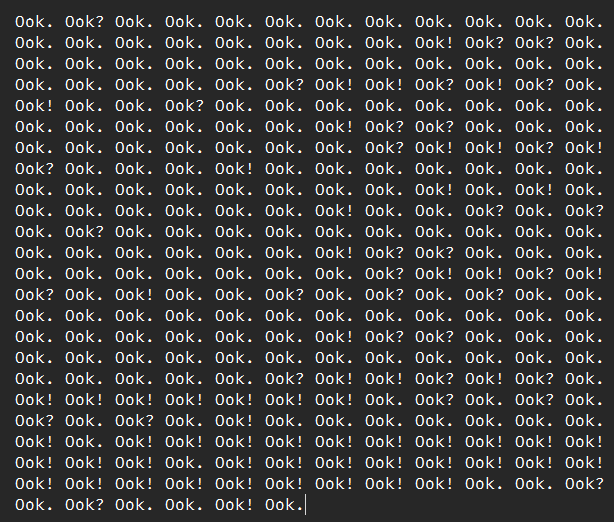
\includegraphics[width=0.5\textwidth]{Figures/ook.png} % Include the figure
	\caption{\textbf{\textit{Hello, World!}} w języku Ook!}
\end{figure}

\subsection{Befunge - program w dwóch wymiarach}
\textbf{Befunge} jest językiem dwuwymiarowym, stworzonym w~1993 roku przez Chrisa Presseya\footnote{\url{https://esolangs.org/wiki/Chris_Pressey}},
którego celem było stworzenie języka tak trudnego do kompilowania jak to możliwe.
Kod każdego programu jest rozłożony na dwuwymiarowej siatce instrukcji, a podczas wykonywania program może przemieszczać się w każdym kierunku
tej dwuwymiarowej płaszczyzny. Prostokątna siatka złożona jest ze znaków zakodowanych w reprezentacji \textbf{ASCII} - każdego reprezentującego daną instrukcję.
Wskaźnik instrukcji zaczyna zawsze z ustalonej lokalizacji - lewy górny narożnik pola instrukcji; i domyślnie przechodzi w ustalonym kierunku - w prawo;
jeśli napotka on instrukcje, to są one wykonywane.
\subsubsection{Etymologia nazwy Befunge}
\par Nazwa \textit{befunge} wywodzi się z błędu typograficznego, polegającego na niepoprawnym zapisaniu słowa \textit{before} przez
Curtisa Colemana o 4 nad ranem na jednym z systemów chatowych BBS\cite{esolangWiki:befunge}\dots
\par Zawiera w sobie słowo "Funge", oznaczające kategorię języków, w których programy reprezentowane są w przestrzeniach metrycznych z układem
współrzędnych używanym do położenia instrukcji - czyli dokładnie tak, jak dzieje się to w tym języku.\\
Przykładowo nieskończona pętla w 2D wyglądać może tak:
\begin{sexylisting}{Nieskończona pętla w Befunge}
>v
^<
\end{sexylisting}
A prosty program \textbf{\textit{Witaj PP!}} tak:
\begin{sexylisting}{\textbf{\textit{Witaj PP!}} w Befunge}
"!PP jatiW">:v
           |,<
           @
\end{sexylisting}
Program ten można rozbić na poszczególne części:
\begin{enumerate}
	\item znakiem \textbf{"} rozpoczynamy pobieranie ciągu znaków (zapisujemy na stos) do następnego znaku \textbf{"}
	\item przechodzimy w prawo \textbf{>} i pobieramy znak ze stosu~\textbf{:}
	\item przechodzimy na dół (kolejno \textbf{v} \textbf{<}) i wypisujemy znak w reprezentacji ASCII dzięki \textbf{,}
	\item napotykamy instrukcję IF pionową (\textbf{|}) - jeśli wartość pobrana ze stosu to 0, zejdź na \textbf{dół}, jeśli nie, to idź na \textbf{górę}
	\item jeśli program doszedł do \textbf{@} to kończy wykonywanie;
\end{enumerate}

\subsection{INTERCAL - pionierski język ezoteryczny}
INTERCAL jako język programowania został stworzony 26 maja 1972 przez \underline{Donalda R. Woodsa} oraz
\underline{Jamesa M. Lyona} w uniwersytecie Princeton. Jego twórcy mieli jedną aspirację - stworzyć
język, który nie ma nic wspólnego z żadnym innym ważnym i popularnym językiem programowania.
Mieli oni na myśli takie języki jak \textit{FORTRAN}, \textit{BASIC}, \textit{COBOL}, \textit{ALGOL} i tym podobne.
Pełna nazwa języka to \textit{"Compiler Language With No Pronounceable Acronym"}, która z wiadomych powodów została skrócona do
\textbf{"INTERCAL"}\cite{woods1973intercal}.
\par Pisanie jakiegokolwiek programu w tym języku może być bardzo uciążliwe dla potencjalnego programisty. Nawet tak prosty program jak
\textbf{\textit{Hello, World!}} może przysporzyć wiele problemów:
\begin{sexylisting}{\textbf{\textit{Hello, World!}} w INTERCALu}
DO ,1 <- #13
PLEASE DO ,1 SUB #1 <- #238
DO ,1 SUB #2 <- #108
DO ,1 SUB #3 <- #112
DO ,1 SUB #4 <- #0
DO ,1 SUB #5 <- #64
DO ,1 SUB #6 <- #194
PLEASE DO ,1 SUB #7 <- #48
DO ,1 SUB #8 <- #26
DO ,1 SUB #9 <- #244
PLEASE DO ,1 SUB #10 <- #168
DO ,1 SUB #11 <- #24
DO ,1 SUB #12 <- #16
DO ,1 SUB #13 <- #162
PLEASE READ OUT ,1
PLEASE GIVE UP
\end{sexylisting}
Na pierwszy rzut oka nie wiadomo, co dokładnie program ten wykonuje.
Istotny tu jest fakt, że komenda \textbf{READ OUT} wypisuje zawartość tablicy, która została akurat zapisana w punkcie \textbf{,1} (linia 15).
Znak przecinka \textbf{,} mówi kompilatorowi, że ma do czynienia z tablicą 16-bitowych liczb całkowitych. Wartości tablicy są wypisywane na wyjście
pojedynczo, od lewej do prawej. By móc zdecydować, który znak należy wypisać, bazując na i-tej pozycji tablicy, 
kompilator przeprowadza operacje według danego algorytmu\cite{intercal:algorithm}:
\begin{enumerate}
	\item odwróć binarnie kod ASCII poprzednio wyświetlonego znaku (dla pierwszego znaku będzie to 0)
	\item pobierz i-ty element tablicy
	\item odejmij wartość pobranego elementu (2.) od odwróconego binarnie znaku (1.)
	\item odwróć binarnie otrzymaną wartość (3.) uzyskując zapisany w reprezentacji ASCII znak do wyświetlenia na i-tej pozycji;
\end{enumerate}

\subsection{Malbolge - diabelski język}
\textbf{Malbolge} jest znany jako jeden z najbardziej ezoterycznych językó programowania. Jest też również często potocznie nazywany
\textit{"Językiem programowania pochodzącym z PIEKŁA"}. Jego nazwa wywodzi się z \textit{Malebolge}, 
nazwy ósmego kręgu piekła w \textit{Boskiej Komedii} Dantego\footnote{\url{https://wolnelektury.pl/katalog/lektura/boska-komedia-pieklo/}},
zarezerwowanego dla sprawców przestępstw i oszustów.
Trudność użytkowania tego języka wywodzi się z \cite{sakai2010introduction}:
\begin{itemize}
	\item restrykcyjnych instrukcji;
	\item podmian instrukcji w trakcie wykonywania;
	\item restrykcji wczytywanych danych;
\end{itemize}

Najłatwiej można to zauważyć, analizując kod programu \textbf{\textit{Hello, World!}}\footnote{\url{https://gist.github.com/kspalaiologos/a1fe6913aaff8edea515b4af385368fe}}:
\begin{sexylisting}{\textbf{\textit{Hello, World!}} w Malbolge}
(=<`#9]~6ZY327Uv4-QsqpMn&+Ij"'E%e{Ab~w=_:]Kw%o44Uqp0/Q?xNvL:`H%c#DD2^WV>gY;dts76qKJImZkj
\end{sexylisting}

Jeśli dana instrukcja nie mieści się w przedziale 33-126 (wartości binarnej danego znaku) to wykonywanie się programu jest kończone.
W innym przypadku, by sprecyzować dokładnie, jaka instrukcja zostanie wykonana, wartość wskazywana przez dany rejestr C jest dodawana do siebie,
a następnie wynik ten jest dzielony przez 94 w celu otrzymania reszty z dzielenia. Malbolge składa się z 8 instrukcji, każdej przypisanej do
innej wartości reszty z dzielenia danego znaku:
\begin{table}[H]
	\begin{center}
		\begin{tabular}{| >{\centering}p{1.8cm} | >{\centering}p{5cm}|}
			\hline
			\textbf{(C+[C])\%94} & \textbf{Opis} \tabline
			4 & Ustawia wskaźnik kodu na wartość wskazywaną przez bieżący wskaźnik danych \tabline
			5 & Wyświetla znak w formacie ASCII (wartość A\%256) \tabline
			23 & Pobiera znak i zapisuje go do rejestru A \tabline
			39 & Obraca liczbę o najmniej znaczący bit (np. 000211111\underline{\textbf{2}} staje się \underline{\textbf{2}}000211111). Zapisuje wynik w A i wskaźniku danych \tabline
			40 & Ustaw wskaźnik danych na wartość wskazywaną przez niego \tabline
			62 & Wykonaj \textit{szaloną} operację ze wskaźnikiem [d] oraz rejestrem A \tabline
			68 & Nic nie rób \tabline
			81 & Zakończ program \tabline
			jakakolwiek inna wartość & Patrz \textbf{wartość 68} \tabline
		\end{tabular}
	\end{center}
	\caption{\centering Spis instrukcji języka \textbf{Malbolge}}
	\label{tab:malbolge!Instrukcje}
\end{table}

W \textbf{Tabeli 5} (\textbf{wartość 62}) wspomniano o tak zwanej \textit{szalonej operacji}:

% Please add the following required packages to your document preamble:
% \usepackage{multirow}
\begin{table}[H]
	\begin{center}
	\begin{tabular}{|cc|ccc|}
	\hline
	\multicolumn{2}{|c|}{\multirow{2}{*}{}}                      & \multicolumn{3}{c|}{\textbf{A}}                                                \\ \cline{3-5} 
	\multicolumn{2}{|c|}{}                                       & \multicolumn{1}{c|}{\textit{\textbf{0}}} & \multicolumn{1}{c|}{\textit{\textbf{1}}} & \textit{\textbf{2}} \\ \hline
	\multicolumn{1}{|c|}{\textbf{}}        & \textit{\textbf{0}} & \multicolumn{1}{c|}{1}          & \multicolumn{1}{c|}{0}          & 0          \\ \cline{2-5} 
	\multicolumn{1}{|c|}{\textbf{{[}D{]}}} & \textit{\textbf{1}} & \multicolumn{1}{c|}{1}          & \multicolumn{1}{c|}{0}          & 2          \\ \cline{2-5} 
	\multicolumn{1}{|c|}{}                 & \textit{\textbf{2}} & \multicolumn{1}{c|}{2}          & \multicolumn{1}{c|}{2}          & 1          \\ \hline
	\end{tabular}
	\end{center}
	\caption{\centering Tabela \textit{szalonej operacji} języka \textbf{Malbolge}}
	\label{tab:malbolge!crazyOps}
\end{table}

Polega ona na zamianie bitów rejestru A oraz wskaźnika [D], a następnie wpisania do obu rejestrów wyniku operacji,
np. instrukcja (zaprezentowana za pomocą \textit{crz} dla lepszej czytelności) \textbf{crz 0001112220, 0120120120} da wynik \underline{1001022211}.

\subsection{ArnoldC - terminator wśród ezoteryków}
Język bazujący na sławnych, tak zwanych "one-linerach", Arnolda Schwarzeneggera\footnote{Większość cytatów można znaleźć tutaj: \url{https://youtu.be/ybJWKZB0Erk}}, stworzony przez fińskiego programistę Lauri Hartikkego\footnote{PROFIL: \url{https://github.com/lhartikk}; PROJEKT: \url{https://github.com/lhartikk/ArnoldC} \label{ArnoldSource}} 
w 2013 roku. Składnia samego języka jest znacznie rozbudowana w porównaniu do wcześniejszych przykładów, natomiast jednymi z ciekawszych i bardziej zabawnych kwestii, 
a raczej instrukcji tego języka są:
\begin{table}[H]
	\begin{center}
		\begin{tabular}{| >{\centering}p{4.3cm} | >{\centering}p{3.2cm} |}
			\hline
			\textbf{Instrukcja} & \textbf{Znaczenie} \tabline
			@I LIED & False \tabline
			@NO PROBLEMO & True \tabline
			BECAUSE I'M GOING TO SAY PLEASE & If \tabline
			BULLSHIT & Else \tabline
			YOU HAVE NO RESPECT FOR LOGIC & EndIf \tabline
			STICK AROUND & While \tabline
			CHILL & EndWhile \tabline
			HE HAD TO SPLIT & / \tabline
			YOU ARE NOT YOU YOU ARE ME & == \tabline
			LISTEN TO ME VERY CAREFULLY & DeclareMethod \tabline
			I\textquotesingle LL BE BACK & Return \tabline
			HASTA LA VISTA, BABY & EndMethodDeclaration \tabline
			DO IT NOW & CallMethod \tabline
			YOU SET US UP & SetInitialValue \tabline
			IT\textquotesingle S SHOWTIME & BeginMain \tabline
			YOU HAVE BEEN TERMINATED & EndMain \tabline
			TALK TO THE HAND & Print \tabline
			I WANT TO ASK YOU A BUNCH OF QUESTIONS AND I WANT TO HAVE THEM ANSWERED IMMEDIATELY & ReadInteger \tabline
			WHAT THE FUCK DID I DO WRONG & ParseError \tabline
		\end{tabular}
	\end{center}
	\caption{\centering Tabela wybranych instrukcji języka \textbf{ArnoldC}}
	\label{tab:arnoldC!instrukcje}
\end{table}
Spis wszystkich instrukcji możliwy jest to odnalezienia na stronie projektu na profilu GitHub twórcy\footref{ArnoldSource}.
\par Bardzo prosty do napisania jest również klasyczny program \textbf{\textit{Witaj PP!}}:
\begin{sexylisting}{\textbf{\textit{Witaj PP!}} w ArnoldC}
IT'S SHOWTIME
TALK TO THE HAND "Witaj PP!"
YOU HAVE BEEN TERMINATED
\end{sexylisting}
Istotnym jest, że każda kolejna komenda musi zostać zapisana od nowej linii, zatem kod napisany w taki sposób nie zadziała\cite{esolangWiki:arnoldC}:
\begin{sexylisting}{Niepoprawny kod w ArnoldC}
GET TO THE CHOPPER x HERE IS MY INVITATION y KNOCK KNOCK z ENOUGH TALK
\end{sexylisting}

\subsection{Chef - książka kucharska dla programistów}		% IDEA: a może "gotowanie"?
Język stworzony przez Davida Morgana-Mara w 2002 roku.
Według opisu ze strony głównej języka "\textbf{Chef} to język programowania, w którym pisane programy wyglądają jak przepisy kulinarne"\footnote{"Chef is a programming language in which programs look like recipes.", \url{https://www.dangermouse.net/esoteric/chef.html}, uzyskano dostęp 26.06.2022}.\\
Zasady pisania w Chefie są następujące\cite{eso:ChefHomepage}:
\begin{itemize}
	\item Program nie tylko powinien generować poprawne wartości wynikowe, ale powinien być również łatwy do przyrządzenia i smaczny!
	\item Przepisy mogą być dostępne dla kucharzy dysponujących różnym budżetem;
	\item Jednostki w przepisach muszą być zdefiniowane w systemie metrycznych, ale dopuszczalne jest użycie tradycyjnych miar kucharskich, takich jak \textit{szklanki} (ang. cups), czy \textit{łyżki stołowe} (ang. tablespoons).
\end{itemize}

\subsubsection{Koncepty zawarte w języku}
\begin{itemize}
	\item \textbf{Ingredients} - Składniki przechowują indywidualne wartości używanych danych. Płynne składniki są interpretowane jako znaki Unicode, a suche, bądź niesprecyzowane składniki są wyświetlane jako liczby.
	\item \textbf{Mixing Bowls and Baking Dishes} - składniki w tej strukturze są uporządkowane w danej kolejności - struktura działająca na zasadzie stosu "naleśników amerykańskich"\footnote{"like a stack of pancakes", \url{https://www.dangermouse.net/esoteric/chef.html}, uzyskano dostęp 26.06.2022} z pewnymi restrykcjami:
	\begin{itemize}
		\item nowe \textbf{składniki} są wkładane na górę stosu
		\item usuwanie \textbf{składników} polega na ściąganiu składnika z góry stosu
		\item jeśli zmieni się wartość \textbf{składnika}, to nie wpływa ona na wartość zapisaną w \textbf{Mixing Bowl}, czy \textbf{Baking Dish}
		\item wartości zapisane na stosie utrzymują swoje \textit{mokre} lub \textit{suche} właściwości;
	\end{itemize}
\end{itemize}

\subsubsection{Elementy składni}
Następujące elementy pojawiają się w przepisach, niektóre z nich są opcjonalne. Każdy pojedynczy element musi być przedstawiony w ukazanej kolejności, z pustą linią pomiędzy każdym elementem:
\begin{enumerate}
	\item \textbf{Tytuł przepisu} - opisuje pokrótce działanie programu; zawsze w pierwszej linii programu, zakończony kropką;
	\item \textbf{Komentarze} - \textit{opcjonalne}, pisanie w formie paragrafu po tytule;
	\item \textbf{Lista składników} używanych przez program. \textit{Opcjonalna}. Składnia wygląda następująco:\\
		\textsc{Ingredients.} \\
		\textsc{[wartość] [[typ-miary] miara] nazwa}\\
		\textsc{[kolejne składniki]}
	\begin{itemize}
		\item \textbf{g | kg | pinch[es]} - \textit{suche} miary
		\item \textbf{ml | l | dash[es]} - \textit{mokre} miary
		\item \textbf{cup[s] | teaspoon[s] | tablespoon[s]} - miary obu rodzajów
	\end{itemize}
	Opcjonalnie można określić jeszcze \textsc{typ-miary}: \textbf{heaped | level}, określa on miary \textit{suche};
	Wartości składników, których nazwy się powtarzają, są nadpisywane;
	\item \textbf{Czas przyrządzenia} jest \textit{opcjonalny}. Czas jest liczbą.\\
	\textsc{Cooking time: \textit{czas} (\textit{godzin[y]} | \textit{minut[y]}).}
	\item \textbf{Temperatura piekarnika} jest \textit{opcjonalna}. Niektóre przepisy wymagają pieczenia.\\
	\textsc{Pre-heat oven to \textit{temp} degrees Celsius.}
	\item \textbf{Metody} zawierają faktyczne instrukcje dotyczące przepisu. Każda metoda zapisana jest w danej sentencji. Ignorowane są znaki nowego wiersza.\\
	\textsc{Method.}\\
	\textsc{\textit{składnia danej metody}}
	\item \textbf{Serwowanie}, ostatnie twierdzenie w przepisie.\\
	\textsc{Serves \textit{liczba-gości}}
	\begin{itemize}
		\item wyświetla zawartość \textbf{Baking Dish}, jednocześnie usuwając ze stosu jego składniki, dopóki nie będzie puste. Zaczynając od naczynia pierwszego, przechodzi do kolejnych, dopóki wszystkie naczynia nie zostaną wyświetlone.
	\end{itemize}
	Jest to wartość \textit{opcjonalna}, ale wymagana, jeśli przepis ma wyświetlić cokolwiek.
\end{enumerate}

Program \textbf{\textit{Hello, world!}} napisany w tym języku wygląda bardzo smakowicie\footnote{\url{https://www.dangermouse.net/esoteric/chef_hello.html}, uzyskano dostęp 26.06.2022}:
\begin{sexylisting}{\textbf{\textit{Hello, world!}} w Chef}
Hello World Souffle.

This recipe prints the immortal words "Hello world!", in a basically brute force way. It also makes a lot of food for one person.

Ingredients.
72 g haricot beans
101 eggs
108 g lard
111 cups oil
32 zucchinis
119 ml water
114 g red salmon
100 g dijon mustard
33 potatoes

Method.
Put potatoes into the mixing bowl. Put dijon mustard into the mixing bowl. Put lard into the mixing bowl. Put red salmon into the mixing bowl. Put oil into the mixing bowl. Put water into the mixing bowl. Put zucchinis into the mixing bowl. Put oil into the mixing bowl. Put lard into the mixing bowl. Put lard into the mixing bowl. Put eggs into the mixing bowl. Put haricot beans into the mixing bowl. Liquefy contents of the mixing bowl. Pour contents of the mixing bowl into the baking dish.

Serves 1.
\end{sexylisting}

\subsection{Unreadable - aż za bardzo nieczytelny}
\textbf{Unreadable} jest językiem ezoterycznym powstałym dzięki użytkownikowi \textit{TehZ}\footnote{\url{https://esolangs.org/wiki/User:TehZ}}. Jest to jeden z języków, tak jak INTERCAL, stworzonych po to, by być jak najmniej czytelne i zrozumiałe dla programisty i czytelnika. Ten język jest natomiast trudniejszy od poprzedników w takim sensie, że bazuje on na dwóch bliźniaczych znakach, których zapis za pomocą wielu zestawów czcionek jest nie odróżnienia dla człowieka - rozróżnić je można tylko za pomocą reprezentacji binarnej. Są to znaki apostrofu oraz cudzysłowu:
\begin{table}[H]
	\begin{center}
	\begin{tabular}{lr}
	\textbf{'} & \textbf{"}
	\end{tabular}
	\end{center}
\end{table}
Pisząc programy w tym języku nie wolno używać spacji, ani znaków nowego wiersza.
Co ciekawe, \textbf{Unreadable} jest językiem Turing-kompletnym, a jego składnia zawiera zaledwie 10 instrukcji\cite{esolangWiki:unreadable}:
%tabela instrukcji Unreadable
\begin{table}[H]
	\begin{center}
		\begin{tabular}{| >{\centering}p{2cm} | >{\centering}p{5cm}|}
			\hline
			\textbf{Instrukcja} & \textbf{Opis} \tabline
			'"X & Wyświetl X jako znak Unicode i zwróć wartość X \tabline
			'""X & Zwróć X+1 \tabline
			'""" & Zwróć 1 \tabline
			'""""XY & Wykonaj X i Y, zwróć wartość zwracaną przez Y\tabline
			'"""""XY & Wykonaj Y, gdy X != 0 i zwróć ostatni zapisany wynik\tabline
			'""""""XY & Przypisz wartość X do Y i zwróć Y \tabline
			'"""""""X & Zwróć wartość X lub 0, jeśli zmienna nigdy nie została zainicjowana \tabline
			'""""""""X & Zwróć X-1 \tabline
			'"""""""""XYZ & Jeśli X != 0: Wykonuj Y, w innym przypadku wykonuj Z. Zwróć wartość $\frac{Y}{Z}$ \tabline
			'"""""""""" & Zwróć pojedynczy znak Unicode wczytywany z wejścia lub -1 - jeśli bufor wejścia został wyczerpany \tabline
		\end{tabular}
	\end{center}
	\caption{\centering Spis instrukcji języka \textbf{Unreadable}}
	\label{tab:unreadableInstrukcje}
\end{table}

Zgodnie z opisem tego języka, każdy program jest bardzo nieczytelny dla zwykłego użytkownika, a dobrym przykładem jest zwykły program wyświetlający napis \textbf{\textit{Hello World}}\footnote{\url{https://esolangs.org/wiki/Talk:Unreadable}, uzyskano dostęp 26.06.2022}:
\begin{figure}[H] % [H] forces the figure to be placed exactly where it appears in the text
	\centering % Horizontally center the figure
	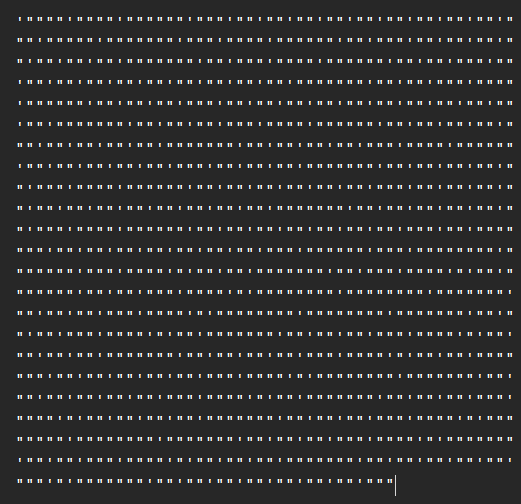
\includegraphics[width=0.5\textwidth]{Figures/unreadable.png} % Include the figure
	\caption{\textbf{\textit{Hello World}} w języku Unreadable}
\end{figure}

\subsection{Whitespace - nieczytelny, ale potężny}
"Niematerialność jest powtarzającym się motywem języków ezoterycznych, być może poprzez fakt, iż języki są praktycznie niczym - zestawem zasad, bez żadnej szczególnej implementacji."\cite{Temkin_2017:articleAll}
\\
\par Najlepszym przykładem takich języków jest \textbf{Whitespace}, stworzony w 2003 roku przez Edwina Bradiego\footnote{\url{https://esolangs.org/wiki/Edwin_Brady}} oraz Chrisa Morrisa, w pełni funkcjonalny język kodowany za pomocą JEDYNIE 3 znaków białych:
\textit{spacji}, \textit{tabulatora}, \textit{znaku nowego wiersza - Entera}.
\par Dzięki takim właściwościom plik zawierający program napisany w tym języku, może sprawiać wrażenie pustego.\\
(!) Co ciekawe, nawet Bjarne Stroustroup - twórca języka C++ - zasugerował dodanie możliwości przeciążania znaków białych, co byłoby równoważne z możliwością przypisywania danych akcji, które mogłyby być wykonywane przy użyciu tych znaków. 
Przykładowo mnożenie dwóch liczb bez użycia znaku mnożenia (\textbf{*}).

\subsubsection{Składnia języka Whitespace}
Przed każdą komendą należy wpisać tak zwane Parametry Modyfikacji Instrukcji (ang. \textbf{IMP} - Instruction Modification Parameters). Składnia jednej pełnej instrukcji wygląda następująco:
\begin{center}
	\textsc{IMP komenda parametry}
\end{center}
\begin{itemize}
	\item parametry zakończone są znakiem nowego wiersza.
\end{itemize}
%tabela instrukcji IMP - whitespace
\begin{table}[H]
	\begin{center}
		\begin{tabular}{| >{\centering}p{1.8cm} | >{\centering}p{5cm}|}
			\hline
			\textbf{IMP} & \textbf{Rodzaj komendy} \tabline
			[Tab][LF] & I/O \tabline
			[Space] & Manipulacja na stosie \tabline
			[Tab][Space] & Arytmetyka \tabline
			[LF] & Kontrola przepływu \tabline
			[Tab][Tab] & Dostęp do elementów na stosie\tabline
		\end{tabular}
	\end{center}
	\caption{\centering Spis instrukcji IMP języka \textbf{Whitespace}}
	\label{tab:whitespaceIMPInstrukcje}
\end{table}
Podział na komendy i ich reprezentacje w języku:
\begin{itemize}
	\item \textbf{Liczby} - by móc wprowadzić liczbę, najpierw należy określić jej znak
	\begin{itemize}
		\item[-] [SPACE] - dodatnia
		\item[-] [TAB] - ujemna
	\end{itemize}
	Następnie należy wprowadzić liczbę w postaci binarnej
	\begin{itemize}
		\item[-] [SPACE] - 0
		\item[-] [TAB] - 1
	\end{itemize}
	\item \textbf{Manipulacje wejścia/wyjścia}
	\begin{table}[H]
		\begin{center}
			\begin{tabular}{| >{\centering}p{2cm} | >{\centering}p{5cm}|}
				\hline
				\textbf{Komenda} & \textbf{Opis} \tabline
				[Tab][Space] & Wczytaj znak i umieść go na szczycie stosu \tabline
				[Tab][Tab] & Wczytaj liczbę i umieść ją na szczycie stosu \tabline
				[Space][Space] & Wyświetl znak ze szczytu stosu \tabline
				[Space][Tab] & Wyświetl liczbę ze szczytu stosu \tabline
			\end{tabular}
		\end{center}
		\caption{\centering Spis komend I/O języka \textbf{Whitespace}}
		\label{tab:whitespaceIOInstrukcje}
	\end{table}
	\item \textbf{Manipulacja stosu}
	\begin{table}[H]
		\begin{center}
			\begin{tabular}{| >{\centering}p{2cm} | >{\centering}p{5cm}|}
				\hline
				\textbf{Komenda} & \textbf{Opis} \tabline
				[Space] & Wypchnij liczbę na szczyt stosu (parametr \textbf{LICZBA}) \tabline
				[LF][Space] & Zduplikuj element na szczycie stosu \tabline
				[LF][Tab] & Zamień miejscami dwa szczytowe elementy stosu \tabline
				[LF][LF] & Odrzuć element ze szczytu stosu \tabline
				[Tab][Space] & Kopiuj \textit{n-ty} (n - parametr) element stosu na szczyt \tabline
				[Tab][LF] & Usuń \textit{n}-elementów (n - parametr) ze stosu, zachowując ten na szczycie \tabline
			\end{tabular}
		\end{center}
		\caption{\centering Spis komend manipulacji stosem języka \textbf{Whitespace}}
		\label{tab:whitespaceSTACKInstrukcje}
	\end{table}
	\item \textbf{Arytmetyka} - opeacje na dwóch szczytowych elementach, wynik operacji nadpisuje je.
	\begin{table}[H]
		\begin{center}
			\begin{tabular}{| >{\centering}p{2cm} | >{\centering}p{3cm}|}
				\hline
				\textbf{Komenda} & \textbf{Opis} \tabline
				[Space][Space] & Dodawanie\tabline
				[Space][Tab] & Odejmowanie \tabline
				[Space][LF] & Mnożenie \tabline
				[Tab][Space] & Dzielenie całkowite \tabline
				[Tab][Tab] & Dzielenie modulo \tabline
			\end{tabular}
		\end{center}
		\caption{\centering Spis komend arytmetycznych języka \textbf{Whitespace}}
		\label{tab:whitespaceAritmethicInstrukcje}
	\end{table}
	\item \textbf{Kontrola przepływu}
	\begin{table}[H]
		\begin{center}
			\begin{tabular}{| >{\centering}p{2cm} | >{\centering}p{5cm}|}
				\hline
				\textbf{Komenda} & \textbf{Opis} \tabline
				[Space][Space] & Znacznik lokalizacji odwołania w programie (parametr LABEL)\tabline
				[Space][Tab] & Przywołaj podprogram (parametr LABEL) \tabline
				[Space][LF] &  Skocz do znacznika (parametr LABEL)\tabline
				[Tab][Space] & Skocz do znacznika, jeśli szczytowy element == 0 (parametr LABEL)\tabline
				[Tab][Tab] & Skocz do znacznika, jeśli szczytowy element jest ujemny (parametr LABEL) \tabline
				[Tab][LF] & Zakończ funkcję i wróć do miejsca jej wywołania \tabline
				[LF][LF] & Zakończ program \tabline
			\end{tabular}
		\end{center}
		\caption{\centering Spis komend kontroli przepływu języka \textbf{Whitespace}}
		\label{tab:whitespaceFlowControlInstrukcje}
	\end{table}
	\item \textbf{Dostęp do elementów na stosie}
	\begin{table}[H]
		\begin{center}
			\begin{tabular}{| >{\centering}p{2cm} | >{\centering}p{5cm}|}
				\hline
				\textbf{Komenda} & \textbf{Opis} \tabline
				[Space] & Wrzuć wartość na stos \tabline
				[Tab] & Pobierz wartość ze stosu \tabline
			\end{tabular}
		\end{center}
		\caption{\centering Spis komend dostępu do stosu języka \textbf{Whitespace}}
		\label{tab:whitespaceHeapAccessInstrukcje}
	\end{table}
\end{itemize}

Przykładowy program z kolorowaną składnią wyświetlający napis \textbf{\textit{Hello World}}\footnote{\url{https://commons.wikimedia.org/wiki/File:Whitespace_in_vim2.png}, uzyskano dostęp 26.06.2022}:
\begin{figure}[H] % [H] forces the figure to be placed exactly where it appears in the text
	\centering % Horizontally center the figure
	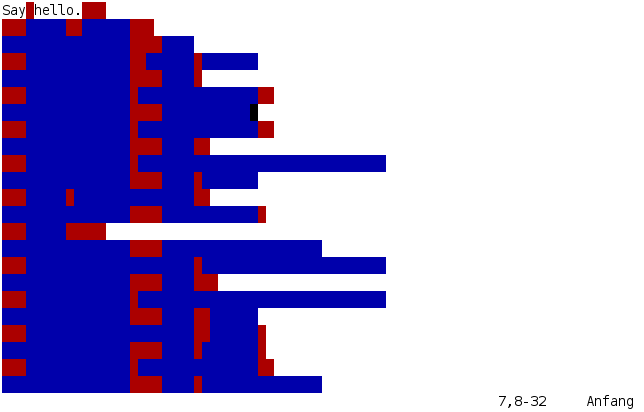
\includegraphics[width=0.5\textwidth]{Figures/whitespace.png} % Include the figure
	\caption{Program wyświetlający napis \textbf{\textit{Hello World}} w języku Whitespace}
\end{figure}
\begin{itemize}
	\item kolorem \textcolor{blue}{niebieskim} zaznaczono znaki tabulatora [TAB]
	\item kolorem \textcolor{red}{czerwonym} zaznaczono znaki spacji [SPACE]
\end{itemize}

\section{Podsumowanie i wnioski}
\par Języki ezoteryczne na pierwszy rzut oka wydają się być bezsensownymi tworami, czasem ciekawymi i intrygującymi, a innym razem frustrującymi zbiorami z pozoru bezsensownych układów znaków, czy bluźnierczych wyrazów.
\par Przyglądając im się coraz uważniej, można natomiast odkryć, jak fascynująca jest nauka i komputer, którym\\ogromna rzesza ludzi na świecie posługuje się codziennie. 
\par Jednym z większych problemów, na jakie wskazują języki ezoteryczne jest ilość komend i jednocześnie wymagana pojemność pamięci, jaka jest potrzebna, by móc przetworzyć ten sam problem programistyczny. Spośród 11 wymienionych i opisanych języków można odnaleźć te, które potrzebują zaledwie \textbf{kilku/kilkunastu bajtów}, by móc wykonać klasyczny program wyświetlający napis \textit{"Hello, World!"}. 
\par Jednocześnie możliwym jest stworzenie takiego programu w innych językach, który jest nie tylko w zupełności nieczytelny dla programisty, ale jednocześnie zajmuje ogromną ilość miejsca. Zalet takich języków należy doszukiwać się natomiast w składni użytej do prezentacji danego problemu. Na przykładzie języka \textbf{Whitespace} można wykazać, że konstruując odpowiednio język kompilatora, można osiągnąć twór, który zawiera w sobie tylko 3 znaki, pozwalający jednocześnie w pełni na użytkowanie go w taki sposób jak inne popularne języki programowania. Jest to również bardzo ważny dowód, ukazujący uniwersalność komputerów użytkowanych we wszelakiej postaci. \par Twórca danego języka ezoterycznego może stworzyć zestaw reguł i reprezentacji składni, który nie będzie w niczym odstawał od zwykłego tekstu beletrystycznego, dramatu, czy przepisu na smaczny suflet czekoladowy, a przy tym program w nim napisany będzie całkowicie wykonywalny.
\par Fascynującym we wszystkich tych pracach jest fakt, że każdy z języków został napisany i przygotowany z pasją i chęcią stworzenia czegoś nowego, innego, dziwnego i trudnego do zrozumienia, ale jednocześnie przemyślanego i dobrze skonstruowanego. 
\par Dzięki takiemu podejściu można wysnuć wniosek, że za pomocą komputera można przedstawić praktycznie wszystko w formie wszelakiej, ale pozwalające uzyskać ten sam wynik końcowy - wystarczy tylko cierpliwość, zaangażowanie, pomysł i dużo wyobraźni.
%%%%%%%%%%%%%%%%%%%%%%%%%%%%%%%%%%%%%%%%%

\phantomsection
\bibliographystyle{unsrt}
\bibliography{bibliography.bib}

\end{document}